\documentclass[a4paper,15pt, oneside]{report}
\usepackage[italian]{babel}
\usepackage[utf8]{inputenc}
\usepackage[a4paper,top=2.5cm,bottom=2.5cm,left=2cm,right=2cm]{geometry}
\usepackage{amssymb}
\usepackage{amsthm}
\usepackage{graphics}
\usepackage{amsfonts}
\usepackage{amsmath}
\usepackage{amstext}
\usepackage{engrec}
\usepackage{rotating}
\usepackage[safe,extra]{tipa}
\usepackage{multirow}
\usepackage{hyperref}
\usepackage{enumerate}
\usepackage{braket}
\usepackage{marginnote}
\usepackage{pgfplots}
\usepackage{cancel}
\usepackage{polynom}
\usepackage{booktabs}
\usepackage{enumitem}
\usepackage{algorithm}
\usepackage{algpseudocode}
\usepackage{framed}
\usepackage{pdfpages}
\usepackage{pgfplots}
\usepackage{fancyhdr}
\usepackage{caption}
\usepackage{subcaption}
\usepackage{setspace}
\usepackage{hyperref}
\usepackage{colortbl}

\usepackage{tikz}\usetikzlibrary{er}\tikzset{multi  attribute /.style={attribute
    ,double  distance =1.5pt}}\tikzset{derived  attribute /.style={attribute
    ,dashed}}\tikzset{total /.style={double  distance =1.5pt}}\tikzset{every
  entity /.style={draw=orange , fill=orange!20}}\tikzset{every  attribute
  /.style={draw=MediumPurple1, fill=MediumPurple1!20}}\tikzset{every
  relationship /.style={draw=Chartreuse2,
    fill=Chartreuse2!20}}\newcommand{\key}[1]{\underline{#1}}
\usetikzlibrary{arrows.meta}
\usetikzlibrary{decorations.markings}
\usetikzlibrary{arrows,shapes, shapes.geometric,backgrounds,petri}
\tikzset{
  place/.style={
    circle,
    thick,
    draw=black
    minimum size=6mm,
  },
  transition/.style={
    rectangle,
    thick,
    fill=black,
    minimum width=8mm,
    inner ysep=2pt
  },
  transitionv/.style={
    rectangle,
    thick,
    fill=black,
    minimum height=8mm,
    inner xsep=2pt
  }
}
\tikzset{elliptic state/.style={draw,ellipse}}

\usetikzlibrary{automata,positioning, calc}

\pagestyle{fancy}
\fancyhead[L,RO]{\slshape \rightmark}
\fancyfoot[C]{\thepage}

\title{Report del progetto di Machine Learning}
\author{Ferrario Tommaso Matr. 869005 (\href{https://github.com/TommasoFerrario18}{@TommasoFerrario18}) \\\\
Terzi Telemaco Matr. 865981(\href{https://github.com/Tezze2001}{@Tezze2001}) \\\\
Vendramini Simone Matr. 866229(\href{https://github.com/simone-vendramini}{@Svendra4MySelf})}
\date{\today}

\pgfplotsset{compat=1.13}

\begin{document}

\maketitle

\newtheorem{teorema}{Teorema}
\newtheorem{dimostrazione}{Dimostrazione}
\newtheorem{definizione}{Definizione}
\newtheorem{esempio}{Esempio}
\newtheorem{osservazione}{Osservazione}
\newtheorem{nota}{Nota}
\newtheorem{corollario}{Corollario}
\tableofcontents
\renewcommand{\chaptermark}[1]{
  \markboth{\chaptername
    \ \thechapter.\ #1}{}}
\renewcommand{\sectionmark}[1]{\markright{\thesection.\ #1}}

\chapter{Introduzione}
Nei capitoli successivi verrà presentato il progetto realizzato per l'esame di
Machine Learning del corso di laurea magistrale in informatica dell'Università
degli Studi di Milano-Bicocca.

L'intero progetto si basa sul riconoscimento della presenza di un tumore al
cervello data l'immagine di una risonanza magnetica.

Il dataset scelto per questo progetto è scaricabile dal seguente
\href{https://www.kaggle.com/datasets/jakeshbohaju/brain-tumor/data}{link} ed è
composto da un insieme di immagini di risonanze magnetiche del cervello di
diversi pazienti e da un file contenete delle features estratte da esse.

Per il riconoscimento del tumore sono stati allenati i seguenti modelli:
\begin{itemize}
    \item \textbf{SVM}: è stato scelto questo modello vista la buona capacità
          teorica nel generalizzare.
    \item \textbf{Gaussian Naive Bayes}: è stato scelto questo modello dal
          momento che permette di modellare le probabilità esplicitamente.
    \item \textbf{Rete neurale}: è stato scelto questo modello per confrontare
          i primi due con una soluzione neurale.
\end{itemize}
L'obiettivo sarà quello di trovare il modello migliore che riduca al minimo i
falsi negativi, mantenendo comunque una buona precisione sui veri negativi. Per
la ricerca sono state effettuate le seguenti operazioni:
\begin{itemize}
    \item \textbf{Analisi esplorativa dei dati}: studio esplorativo del dataset
          utile per effettuare le prime osservazioni sui dati.
    \item \textbf{Riduzione di dimensionalità e preprocessing del dataset}:
          applicazione di diverse trasformazioni del dataset, dalla rimozione
          dei duplicati, fino alla rimozione dei valori costanti. In aggiunta è
          stata ridotta la dimensionalità utilizzando due metodi, il primo
          basato sulla rimozione delle features correlate, il secondo basato
          sull'utilizzo della Principal Component Analysis (PCA). In questa fase
          vengono quindi generati i due dataset.
    \item \textbf{Valutazione dei modelli}: per ciascun dataset si è effettuata
          una valutazione dei modelli in due passi, la prima è una valutazione
          su ciascuna effettuando un allenamento sull'$80\%$ delle istanze e
          valutando sul rimanente $20\%$, la seconda è una $10$-fold stratified
          cross-validation per una valutazione più affidabile e robusta.
          Nella prima valutazione, durante la fase di training si effettua anche
          una $5$-fold stratified cross-validation sul training set, per
          ricercare gli iperparamentri migliori da utilizzare nel modello che
          verrà successivamente valutato nelle due fasi.
    \item \textbf{Confronto tra i vari modelli}: sono stati confrontati tutti
          i modelli sia in merito ai criteri di valutazione, sia in merito ai
          tempi di apprendimento.
\end{itemize}
Sono state effettuate due validazioni a causa della dimensione del dataset,
infatti, vista la sua media dimensione si è deciso di confermare le osservazioni
indotte dalla prima valutazione effettuando una cross-validation con gli
iperparametri trovati nella fase di validazione validazione.

Per concludere, illustriamo la struttura dell'elaborato, la quale si articola
nei seguenti capitoli:
\begin{itemize}
    \item \textbf{Introduzione}: descrizione del dominio e presentazione dei
          modelli che verranno presi in considerazione per questo progetto.
    \item \textbf{Dataset}: descrizione di come è stato costruito il dataset a
          partire dalle immagini, ovvero come sono state ricavate le features, e
          analisi esplorativa.
    \item \textbf{Rete neurale}: descrizione e analisi delle performance della
          rete.
    \item \textbf{SVM}: descrizione e analisi delle performance delle SVM.
    \item \textbf{Gaussian Naive Bayes}: descrizione e analisi delle performance
          per Gaussian Naive Bayes.
    \item \textbf{Analisi dei risultati}: analisi comparata dei risultati tra i
          tre modelli considerati.
    \item \textbf{Conclusioni}: conclusioni sull'elaborato.
\end{itemize}
\chapter{Dataset}
\section{Struttura del dataset}
Il dataset è composto da un set di $3762$ immagini, ognuna delle quali è stata
ottenuta dalla risonanza magnetica del cervello. Ad ogni immagine è stata
associata un etichettata la quale permette di rappresentare la presenza o meno
di un tumore al cervello. Nel dataset è presente una colonna, \textit{Class},
nella quale sono presenti le etichette, ovvero:
\begin{itemize}
      \item \textbf{Presenza del tumore}: $T = 1$
      \item \textbf{Assenza del tumore}: $T = 0$
\end{itemize}

Oltre alla colonna \textit{Class}, il dataset è composto da altre $13$ colonne,
nelle quali sono presenti le feature calcolate sulle immagini. Tali features sono state
ottenute calcolando i \textbf{momenti Hu} sulle immagini della risonanza magnetica.
I momenti Hu catturano le informazioni di base sull'immagine come l'area
dell'oggetto, il centroide, l'orientamento e altre proprietà.

Gli attributi di cui è composto il dataset possono essere suddivisi in 2 gruppi\cite{explanation-features}:
\begin{enumerate}
      \item \textbf{First Order Features}: forniscono informazioni legate alle
            distribuzione dei livelli di grigio dell'immagine. Queste features
            corrispondono alle statistiche descrittive calcolate sui valori di
            ciascun pixel dell'immagine. Le statistiche descrittive calcolate sono:
            \begin{itemize}
                  \item \textbf{Media}
                  \item \textbf{Varianza}
                  \item \textbf{Deviazione standard}
                  \item \textbf{Indice di asimmetria}
                  \item \textbf{Indice di kurtosis}
            \end{itemize}
      \item \textbf{Second Order Features}: forniscono informazioni a livello di
            composizione della texture dell'immagine.
            \begin{itemize}
                  \item \textbf{Contrasto}: misura la variazione locale dei livelli
                        di grigio dei pixel. Maggiore sarà il valore allora maggiore
                        sarà il contrasto dell'immagine.
                  \item \textbf{Energia}: misura l'eterogeneità o la variazione
                        dell'intensità dell'immagine. Più piccolo è il valore allora
                        meno variazioni di intensità e più omogenea sarà la texture,
                        al contrario, più la texture è irregolare allora maggiore
                        sarà il valore.
                  \item \textbf{ASM}: misura quanto sono distribuiti uniformemente i
                        livelli di grigio nell'immagine. Più i livelli di grigio sono
                        uniformemente distribuiti minore sarà il valore dell'indice.
                  \item \textbf{Entropia}: misura la randomicità dei livelli di
                        grigio, quindi più piccolo è il valore, più la texture
                        sarà uniforme.
                  \item \textbf{Homogeneous}: misura secondaria del contrasto. Più
                        alto sarà l'indice allora minore sarà il contrasto dell'immagine.
                  \item \textbf{Dissimilarity}: misura quanto spesso differenti
                        combinazioni dei valori di intensità dei pixel occorrono
                        nell'immagine. Un valore alto indica che l'immagine ha una
                        maggior variazione delle intensità dei pixel vicini,
                        quindi più complessa sarà la texture.
                  \item \textbf{Correlation}: misura la correlazione tra pixel nelle
                        due diverse direzioni.
                  \item \textbf{Coarseness}: misura quanto l'immagine è composta da
                        regioni di intensità omogenea, ovvero quanto è granulare o
                        fine la texture.
            \end{itemize}
\end{enumerate}
\section{Analisi descrittiva}\label{sec:analisi-descrittiva}
Il dataset è formato da un totale $3762$ istanze, ciascuna delle quali è descritta
da $15$ attributi così suddivisi:
\begin{itemize}
      \item $13$ rappresentano le feature calcolate sulle immagini della risonanza
            magnetica. Tutti questi attributi sono di tipo \textit{float}.
      \item $1$, ovvero l'attributo \textit{Image}, rappresenta l'identificativo
            dell'immagine a cui si riferisce l'istanza.
      \item $1$, ovvero l'attributo \textit{Class}, rappresenta l'etichetta associata
            all'immagine. Questo attributo è stato convertito da \textit{intero} a
            \textit{categorico} per poter effettuare la classificazione.
\end{itemize}

Caricato il dataset, è stato eseguito un controllo per verificare che non ci fossero
valori nulli. In questo caso non sono stati trovati valori nulli, quindi non è
stato necessario eseguire alcuna operazione per la gestione di tali valori.
% Todo: controllare se nel dataset ci sono valori duplicati

Successivamente, si è proceduto con il calcolo delle statistiche descrittive per
gli attributi numerici presenti nel dataset. Questa operazione ha permesso di
ottenere le informazioni riportate nella tabella \ref{tab:desc-stat}.

\begin{table}[h!]
      \begin{subtable}[h]{1\textwidth}
            \centering
            \resizebox{\textwidth}{!}{\begin{tabular}{c|c c c c c c c c c c}
                        \hline
                        \rowcolor[HTML]{EFEFEF} \cellcolor[HTML]{EFEFEF}\textbf{} & \textbf{Mean} & \textbf{Variance} & \textbf{Standard Deviation} & \cellcolor[HTML]{EFEFEF}\textbf{Entropy} & \textbf{Skewness} & \textbf{Kurtosis} \\ \hline
                        \textbf{count}                                            & 3762          & 3762              & 3762                        & 3762                                     & 3762              & 3762              \\
                        \textbf{mean}                                             & 9.488890      & 711.101063        & 25.182271                   & 0.073603                                 & 4.102727          & 24.389071         \\
                        \textbf{std}                                              & 5.728022      & 467.466896        & 8.773526                    & 0.070269                                 & 2.560940          & 56.434747         \\
                        \textbf{min}                                              & 0.078659      & 3.145628          & 1.773592                    & 0.000882                                 & 1.886014          & 3.942402          \\
                        \textbf{25\%}                                             & 4.982395      & 363.225459        & 19.058475                   & 0.006856                                 & 2.620203          & 7.252852          \\
                        \textbf{50\%}                                             & 8.477531      & 622.580417        & 24.951560                   & 0.066628                                 & 3.422210          & 12.359088         \\
                        \textbf{75\%}                                             & 13.212723     & 966.954319        & 31.095889                   & 0.113284                                 & 4.651737          & 22.640304         \\
                        \textbf{max}                                              & 33.239975     & 2910.581879       & 53.949809                   & 0.394539                                 & 36.931294         & 1371.640060       \\ \hline
                  \end{tabular}}
            \caption{Statistiche descrittive delle feature \textit{Mean}, \textit{Variance}, \textit{Standard Deviation}, \textit{Entropy}, \textit{Skewness} e \textit{Kurtosis}.}
            \label{tab:primameta}
      \end{subtable}
      \hfill
      \begin{subtable}[h]{1\textwidth}
            \centering
            \resizebox{\textwidth}{!}{\begin{tabular}{c|c c c c c c c c}
                        \hline
                        \rowcolor[HTML]{EFEFEF} \cellcolor[HTML]{EFEFEF}\textbf{} & \textbf{Contrast} & \textbf{Energy} & \textbf{ASM} & \textbf{Homogeneity} & \textbf{Dissimilarity} & \textbf{Correlation} & \textbf{Coarseness} \\ \hline
                        \textbf{count}                                            & 3762              & 3762            & 3762         & 3762                 & 3762                   & 3762                 & 3762                \\
                        \textbf{mean}                                             & 127.961459        & 0.204705        & 0.058632     & 0.479252             & 4.698498               & 0.955767             & 7.458341e-155       \\
                        \textbf{std}                                              & 109.499601        & 0.129352        & 0.058300     & 0.127929             & 1.850173               & 0.026157             & 0.000000e+00        \\
                        \textbf{min}                                              & 3.194733          & 0.024731        & 0.000612     & 0.105490             & 0.681121               & 0.549426             & 7.458341e-155       \\
                        \textbf{25\%}                                             & 72.125208         & 0.069617        & 0.004847     & 0.364973             & 3.412363               & 0.947138             & 7.458341e-155       \\
                        \textbf{50\%}                                             & 106.737418        & 0.225496        & 0.050849     & 0.512551             & 4.482404               & 0.961610             & 7.458341e-155       \\
                        \textbf{75\%}                                             & 161.059006        & 0.298901        & 0.089342     & 0.575557             & 5.723821               & 0.971355             & 7.458341e-155       \\
                        \textbf{max}                                              & 3382.574163       & 0.589682        & 0.347725     & 0.810921             & 27.827751              & 0.989972             & 7.458341e-155       \\ \hline
                  \end{tabular}}
            \caption{Statistiche descrittive delle feature \textit{Contrast}, \textit{Energy}, \textit{ASM}, \textit{Homogeneity}, \textit{Dissimilarity}, \textit{Correlation} e \textit{Coarseness}.}
            \label{tab:secondameta}
      \end{subtable}
      \caption{Statistiche descrittive degli attributi}
      \label{tab:desc-stat}
\end{table}

Questa operazione ha permesso di ottenere alcune informazioni sul dataset.
Innanzitutto, ha permesso di osservare che i valori associati agli attributi non
sono standardizzati dal momento che nessun dato ha media $0$ e deviazione
standard $1$.

La standardizzazione delle feature è stata fatta, utilizzando l'equazione
\ref{eq:std-features}, solo per le SVM e il modello neurale, mentre per Gaussian
Bayes la standardizzazione viene fatta in automatico dalla libreria del modello.
\begin{equation}
      F_{\mu, \sigma} = \frac{F - \mu}{\sigma}
      \label{eq:std-features}
\end{equation}

In aggiunta alle statistiche descrittive, per ogni feature si è realizzato un
istogramma attraverso il quale è stato possibile realizzare una prima analisi
visiva sulla distribuzione dei valori. Questa operazione è stata svolta per
verificare se le feature seguono una distribuzione normale.

\textbf{TODO:immagine}

Da questi grafici si evince che le feature \textit{Energy}, \textit{Homogeneity}
e \textit{Coarseness} non seguono una distribuzione normale, a differenza delle
altre feature che possono essere considerate normali. In ogni caso, anche se non
seguono l'ipotesi di normalità, si è deciso comunque di utilizzarli, anche se
stiamo andando contro le assunzioni dei modelli che vogliamo utilizzare. % TODO: non ho capito cosa vuol dire

Da questa analisi, è stato possibile osservare che la feature \textit{Coarseness}
assume valori molto bassi, quindi è stato pensato di convertire questa feature
ad una scala logaritmica, permettendo di aumentare la significatività dei valori.

Nonostante questa operazione, la feature \textit{Coarseness} presenta una deviazione
standard pari a circa $0.02$, valore non particolarmente significativo, quindi
questo ci ha permesso di escludere questa feature perché sicuramente non sarà la
feature più discriminante.

Oltre all'analisi descrittiva delle feature, è stato eseguito anche un analisi
sulle etichette, ovvero sulle classi. Questo è stato fatto per verificare se le
classi sono bilanciate, ovvero se il numero di esempi positivi è simile al numero
di esempi negativi.

In questo caso, realizzando un istogramma, riportato in figura \ref{fig:dist-classi},
che rappresenta le frequenze assolute delle classi. Da questo si può notare che
la distribuzione di esse è bilanciate, infatti, circa il $55\%$ degli esempi sono
negativi (assenza del tumore), contro circa il $45\%$ degli esempi sono positivi
(presenza del tumore).

\begin{figure}[!ht]
      \centering
      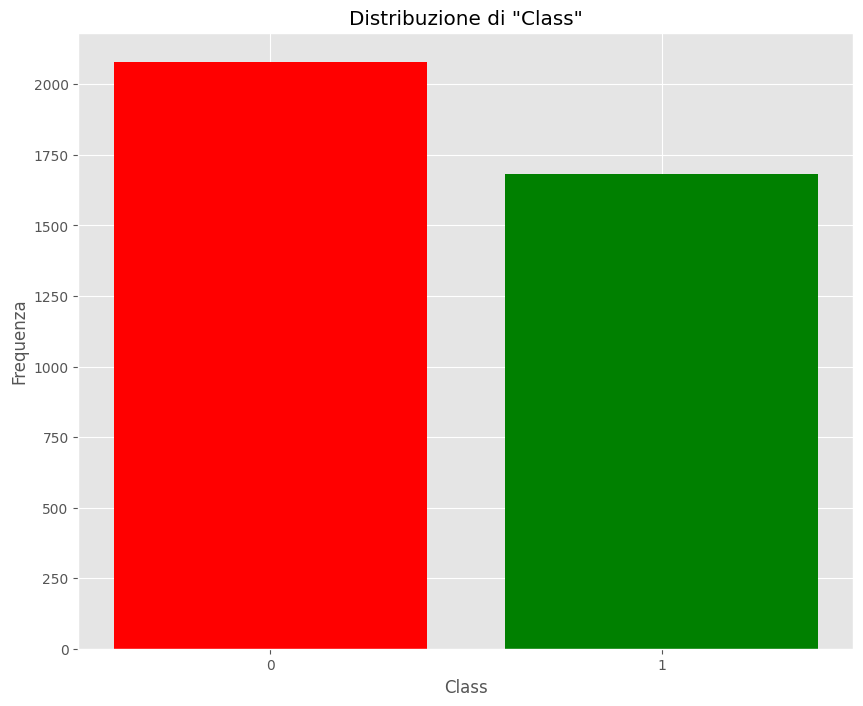
\includegraphics[width=0.5\textwidth]{img/analisi/distribuzioneClassi.png}
      \caption{Distribuzione delle classi}
      \label{fig:dist-classi}
\end{figure}

\textbf{Non è già stato detto prima?}
Successivamente risulta importante analizzare se le distribuzioni si avvicinano
ad una normale standard, di conseguenza sono stati disegnati i barplot delle frequenze
di ciascuna feature. Dai grafici si evince che tutte le feature eccetto \textit{Energy} e
\textit{Homogeneity} sono distribuite normalmente.

Dal barplot delle features creato precedentemente, si possono ottenere ulteriori
informazioni sulla distribuzione potenzialmente normale delle altre feature. Infatti,
la distribuzione della \textit{Standard deviation} è simmetrica, mentre tutte
le altre presentano una asimmetria.

Ricapitolando, da questo primo studio descrittivo è stato modificato il dataset
rimuovendo la feature \textit{Coarseness}.

\textbf{TODO:immagine}

\subsection{Analisi delle correlazioni}
Il passaggio successivo è  stato quello di analizzare le correlazioni tra le feature.
Questo è stato fatto in modo tale da ridurre la dimensionalità dei dati, nello
specifico sono state suddivise le feature in gruppi di feature altamente correlate
tra loro, e in un secondo momento è stata scelta una feature per ogni gruppo.

Per fare ciò, è stata realizzata una matrice di correlazione, riportata in figura
\ref{fig:corr-matrix}, attraverso la quale è stato possibile osservare le correlazioni
tra le feature.

\begin{figure}[!ht]
      \centering
      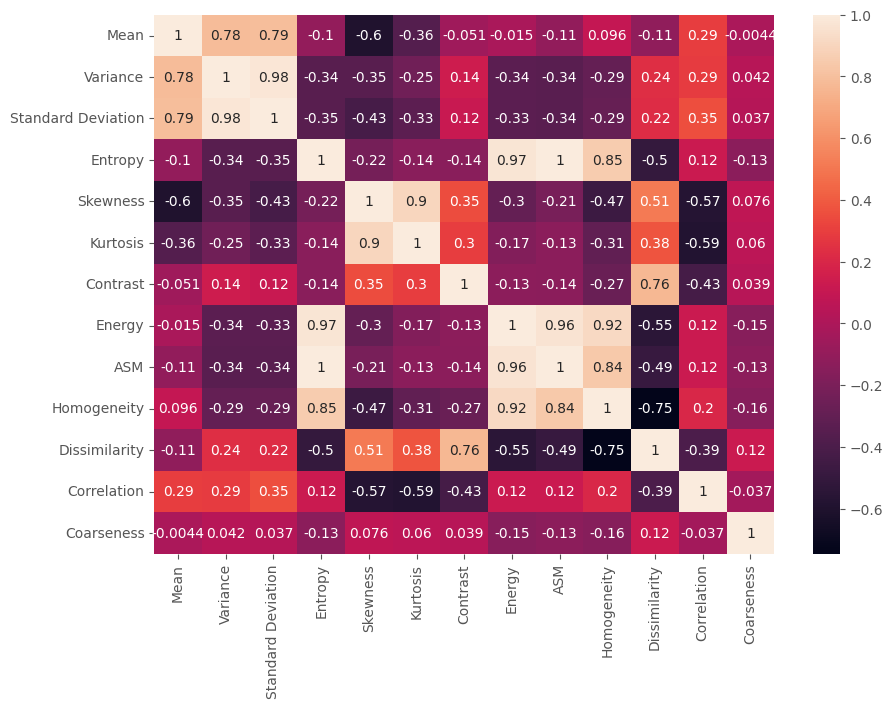
\includegraphics[width=0.5\textwidth]{img/analisi/corr.png}
      \caption{Matrice di correlazione}
      \label{fig:corr-matrix}
\end{figure}

Dall'analisi di questa matrice, si possono osservare diverse correlazioni tra le
feature. Innanzitutto, si può notare una forte correlazione positiva tra le feature
\textit{Mean}, \textit{Variance} e \textit{Standard deviation}. Questa correlazione
è facilmente spiegabile analizzando le immagini prodotte dalle risonanze magnetiche.
Infatti, essendo in bianco e nero, se la media tende a $1$ (colore bianco) allora
la varianza e la deviazione standard aumentano, perché sono presenti diversi
pixel bianchi. Questo comporta che le transizioni dal nero assoluto al bianco
assoluto necessitano di regioni di pixel maggiore rispetto ad una transizione
tra nero assoluto e grigio ($0.5$).

Invece, la correlazione tra varianza è deviazione standard facilmente spiegabile
perché la deviazione standard è la radice quadrata della varianza ($SD[P] = \sqrt{VAR[P]}$).

\textbf{TODO:immagine}

Una seconda forte correlazione positiva si può osservate tra le feature che
misurano l'\textbf{uniformità dei livelli di grigio} dei pixel, più precisamente
tra le feature \textit{Entropy}, \textit{ASM}, \textit{Homogeneity} ed
\textit{Energy}. Queste feature quantificano delle informazioni legate alla
texture dell'immagine, quindi la forte correlazione positiva può essere spiegata
analizzando le texture delle immagini su cui vengono calcolate. Più precisamente
se si ha un valore molto alto della feature \textit{Entropy}, significa che la
texture non è uniforme, ovvero si hanno strutture complesse e irregolari, quindi
meno uniforme sarà la distribuzione dei livelli di grigio, aumentando l'indice
di \textit{ASM}, comportando di conseguenza un aumento delle variazioni di intensità
dei livelli di grigio, aumentando di conseguenza anche l'indice di \textit{Energy},
infine, (\textbf{cosa c'entra Homogeneity?}).

Al tempo stesso, la matrice di correlazione evidenza una forte correlazione positiva
tra gli indici che misurano la \textbf{morfologia della distribuzione}, ovvero
le feature di \textit{Skewness} e \textit{Kurtosis}. Questa dipendenza implica il
fatto che più la distribuzione è leptokurtica (Kurtosis grande), ovvero la frequenza
dei livelli di grigio dei pixel si concentrano interamente vicino alla media/mediana/
moda, allora più grande sarà la Skewness, ovvero maggiore sarà la tendenza ad avere
frequenze di livelli di grigio più vicino al bianco (coda di destra più altra rispetto
alla coda di sinistra).

La matrice della correlazione evidenzia anche una correlazione positiva tra le
feature di \textit{Contrast} e \textit{Dissimilarity}, ovvero maggiore sarà il
contrasto e maggiore sarà la complessità della texture.

In aggiunta dalla matrice si evidenza che le features di \textit{Dissimilarity}
e \textit{Homogeneity} sono correlate negativo, ovvero maggiore sarà il contrasto
allora minore è la complessità della texture.

Dalla correlazione delle features è possibile ridurre la dimensionalità del dataset
considerando sono le seguenti features:
\begin{itemize}
      \item \textbf{Mean}
      \item \textbf{Entropy}
      \item \textbf{Skewness}
      \item \textbf{Contrast}
      \item \textbf{Correlation}
\end{itemize}
A puro scopo didattico è stato pensato di eseguire i modelli non solo sul dataset
semplificato eliminando le correlazioni, ma anche applicando l'algoritmo PCA.

\section{PCA} \label{sec:pca}
Precedentemente è stato presentato un primo modo per ridurre la dimensionalità
dei dati basandoci sull'analisi delle correlazioni. In seguito, è stato pensato
di provare ad utilizzare un metodo di trasformazione delle feature per ridurre
la loro dimensionalità e successivamente analizzare i risultati ottenuti. La
scelta sul metodo da utilizzare è ricaduta su PCA.

Prima di applicare la PCA, è stato necessario standardizzare le feature, questa
operazione è stata fatta per evitare che le feature con varianza maggiore abbiano
un peso maggiore rispetto alle altre. Senza standardizzare le feature, la PCA
potrebbe non essere in grado di trovare le direzioni di massima varianza.

La prima parte dell'analisi è stata quella di trovare il corretto numero di
componenti da utilizzare per la PCA. Questo è stato fatto attraverso
l'osservazione della percentuale di varianza spiegata per ogni componente. Per
svolgere questa operazione sono state utilizzate solamente le feature numeriche
del dataset, quindi sono state escluse le colonne \textit{Image} e \textit{Class}.

Rimosse le colonne non necessarie, è stato possibile computare la PCA utilizzando
la libreria \textit{sklearn} e successivamente è stato possibile osservare la
percentuale di varianza spiegata per ogni componente, riportata in figura \ref{fig:pca}.

\begin{figure}[!ht]
      \centering
      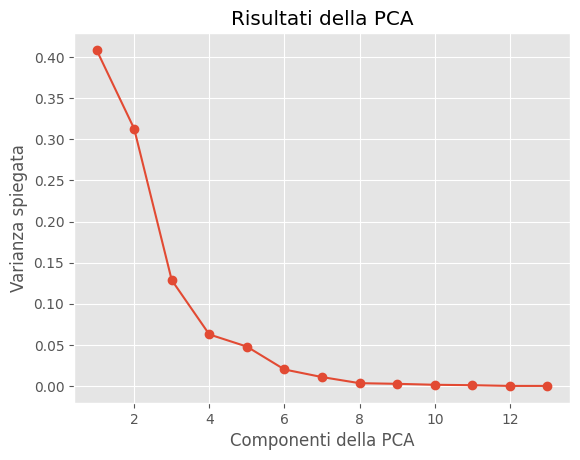
\includegraphics[width=0.45\textwidth]{img/analisi/pcaVarianza.png}
      \caption{Percentuale di varianza spiegata per ogni componente}
      \label{fig:pca}
\end{figure}

Dall'analisi della percentuale di varianza spiegata per ogni componente, si può
osservare che le prime $3$ componenti spiegano circa l'$85\%$ della varianza
dei dati. Questo ci ha permesso di ridurre la dimensionalità del dataset a soli
$3$ attributi, permettendo di rappresentare i dati in uno spazio a $3$ dimensioni.

\begin{figure}[!ht]
      \centering
      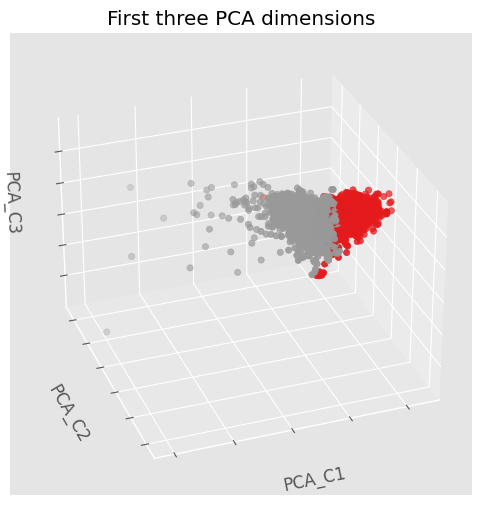
\includegraphics[width=0.4\textwidth]{img/analisi/pcaNuovoDataset.png}
      \caption{Scatter plot a 3 dimensioni}
      \label{fig:pca-3d}
\end{figure}

Dalla figura \ref{fig:pca-3d} si può osservare che i dati ottenuti dalla PCA
sembrano essere separabili con un piano.

\section{Preparazione dei dati per i vari modelli}
In seguito a tutti i ragionamenti precedenti, dal primo dataset sono stati costruiti 
altri due datasets, il primo ridotto mediante la correlazione (Dataset-corr), 
mentre il secondo ridotto mediante PCA (Dataset-pca). La scelta di eseguire i
modelli utilizzando due metodi per ridurre la dimensionalità è stata fatta solo
per scoprire se ha davvero senso, in questo contesto, scomodare un algoritmo di 
riduzione di dimensionalità, come PCA, oppure ci si può limitare solo a considerare
feature non fortemente correlate.

Successivamente su Dataset-corr e Dataset-pca sono state applicate delle operazioni 
di suddivisione degli esempi in due insiemi:
\begin{itemize}
      \item \textbf{training set}: contenente l'$80\%$ degli esempi del dataset e viene
      utilizzato per effettuare la ricerca degli iperparametri migliori e, una volta
      trovati, si riutilizza questo insieme di esempi per allenare il modello con 
      gli iperparametri migliori appena trovati. Per lo studio degli iperparametri
      è stata effettuata una 10-fold cross validation stratified.
      \item \textbf{test set}: contenente l'$80\%$ degli esempi del dataset 
      rimanenti e viene utilizzato per effettuare la valutazione del modello.
\end{itemize}
Logicamente, la suddivisione tra traning set e test set è stata realizzata
in modo strutturato, ovvero nel traing set e nel test set è stato preservato lo 
stesso bilanciamento delle classi presenti nel dataset di partenza, in modo tale 
da evitare di introdurre dei bayes su modello. 

In aggiunta alle operazioni di preprocessing introdotte precedentemente, è stata
applicata anche un'operazione di standardizzazione dei dati definendo due nuovi
dataset: Dateset-corr-std e Dateset-pca-std. La standardizzazione dei dati è
stata necessaria dal momento che sono stati utilizzati dei modelli che assumono
di ricevere in input dei dati standardizzati, come le reti neurali (NN) e le 
support vector machine (SVM).
 
Nella tabella \ref{tab:riassunto-dataset} si può avere una ricapitolazione di
tutti i dataset e delle operazioni effettuate per ottenerli.

\begin{table}[ht]
      \resizebox{\textwidth}{!}{\begin{tabular}{|l|l|l|}
      \hline
      \textbf{Nome del dataset} & \textbf{Operazioni applicate}                                           & \textbf{Utilizzato per i seguenti modelli} \\ \hline
      Dataset-corr              & Riduzione della dimensionalità utilizzando l'analisi della correlazione & Gaussian Naive Bayes              \\ \hline
      Dateset-corr-std          & Dataset-corr con la standardizzazione dei dati                          & SVM e NN                          \\ \hline
      Dateset-PCA               & Dateset-corr-std applicando l'algoritmo PCA                             & Gaussian Naive Bayes              \\ \hline
      Dateset-PCA-std           & Dateset-PCA con la standizzazione dei dati                              & SVM e NN                          \\ \hline
      \end{tabular}}
      \caption{Tabella riassuntiva dei dataset}
      \label{tab:riassunto-dataset}
\end{table}
% ! Struttura presentata nell'introduzione
\chapter{Modelli} \label{ch:modelli}
In questo capitolo verranno presentati i modelli che si è deciso di addestrare 
per svolgere il compito di classificazione. I modelli sono stati scelti in base
ai risultati ottenuti nella fase di analisi esplorativa e in base alle
caratteristiche del dataset. In particolare, si è deciso di addestrare:
\begin{itemize}
    \item \textbf{Support Vector Machine}
    \item \textbf{Gaussian Naive Bayes}
    \item \textbf{Rete Neurale}
\end{itemize} 
Per ognuno di essi verrà presentata una breve descrizione sulla loro struttura
e sulle operazioni che sono state svolte per la loro definizione. In un secondo
momento verranno presentati i risultati ottenuti e verrà fatta una valutazione
sui modelli addestrati.
\section{Support Vector Machine}
% ! Da inserire la parte su SVM
\section{Gaussian Naive Bayes}
Di seguito verrà presentato il processo di addestramento del modello 
\textbf{Gaussian Naive Bayes}. È importante precisare che la scelta di utilizzare 
questo modello è stata fatta con la consapevolezza che non tutte le features 
derivano da una distribuzione normale, andando contro le ipotesi del modello. 
Tuttavia, abbiamo deciso di utilizzarlo in quanto volevamo distaccarci da un 
approccio geometrico e sfruttare un modello probabilistico.
\subsection{Addestramento di Gaussian Naive Bayes}
Come per gli altri approcci, abbiamo deciso di addestrare due modelli, uno su
\texttt{dataset\_corr} e l'altro su \texttt{dataset\_pca}.

La libreria utilizzata per l'implementazione di Gaussian Naive Bayes non 
presenta degli iperparametri da stimare, quindi non è stato necessario effettuare
un processo di ricerca della combinazione migliore.
\section{Rete Neurale}
In questa sezione verrà presentata la \textbf{rete neurale}. Nello specifico, si 
andranno a presentare i passaggi che sono stati effettuati per la realizzazione 
di questo modello, prestando particolare attenzione alla fase di definizione 
della struttura della rete neurale e alla fase di addestramento della stessa.

In questo capitolo tutte le operazioni effettuate sono state realizzate 
utilizzando i dataset standardizzati (\texttt{dataset\_corr\_std} e 
\texttt{dataset\_pca\_std}) presentati nella fase di preparazione dei 
dati \ref{sec:preparazione_dei_dati}.
\subsection{Struttura della rete neurale}
La fase di definizione della struttura della rete neurale è stata effettuata
attraverso una serie di passaggi. Inizialmente, è stata effettuata un'analisi
dei dati in modo tale da selezionare un sottoinsieme di feature le quali sono
state utilizzate come input della rete neurale. Questo sottoinsieme è stato
selezionato in modo tale da garantire che la rete neurale fosse in grado di
discriminare in modo efficace le due classi.

In seguito, è stata effettuata una fase di grid search per valutare la combinazione
migliore di iperparametri per la rete neurale. Questa fase è stata effettuata
attraverso una cross validation a 5 fold, prendendo in considerazione solamente
i dati del training set.

Dai risultati ottenuti dalla fase di analisi e dal dominio del problema, si è
scelto di utilizzare una rete con una struttura di dimensioni ridotte, in modo
tale da ridurre le possibilità che la rete neurale soffra di overfitting.

Per svolgere il compito di classificazione si è scelto di utilizzare una rete
neurale feedforward, la cui struttura, a meno del layer di input e di output, è
stata definita attraverso il processo di grid search.
\subsubsection{Ottimizzazione degli iperparametri}
Come già accennato in precedenza, la ricerca degli iperparametri della rete neurale
è stata effettuata attraverso un processo di grid search. Questo processo ha
permesso di valutare le prestazioni della rete neurale al variare della funzione
di attivazione, del numero di layer nascosti e del numero di neuroni per ogni
layer nascosto.

Visti i risultati ottenuti nella fase di analisi e la volontà di mantenere i
tempi di addestramento bassi, si è scelto di mantenere una struttura di dimensioni
ridotte per la rete neurale. Per questo motivo, l'operazione di grid search è
stata effettuata prendendo in considerazione un numero di neuroni per layer
tra 5, 10 mentre il numero di layer nascosti è stato valutato tra 1 e 2.

Per quanto riguarda la funzione di attivazione, sono state valutate le seguenti
funzioni di attivazione:
\begin{itemize}
    \item \textit{ReLU}
    \item \textit{Leaky ReLU}
    \item \textit{sigmoid}
\end{itemize}

\begin{figure}[!ht]
    \centering
    \begin{subfigure}[b]{0.3\textwidth}
        \centering
        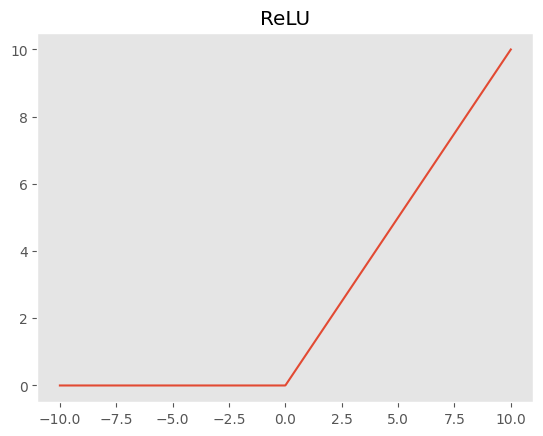
\includegraphics[width=\textwidth]{img/rete/relu.png}
        \caption{ReLU}
        \label{fig:relu}
    \end{subfigure}
    \hfill
    \begin{subfigure}[b]{0.3\textwidth}
        \centering
        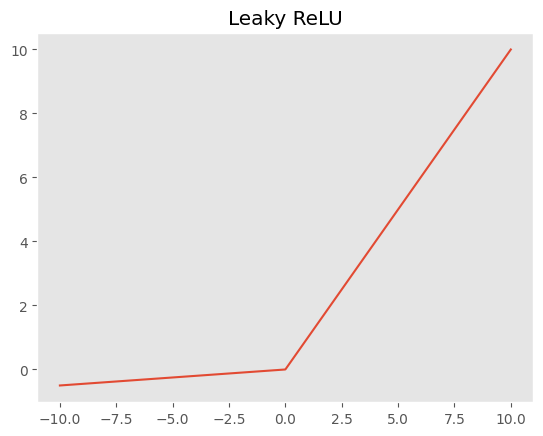
\includegraphics[width=\textwidth]{img/rete/leaky_relu.png}
        \caption{Leaky ReLU}
        \label{fig:leaky-relu}
    \end{subfigure}
    \hfill
    \begin{subfigure}[b]{0.3\textwidth}
        \centering
        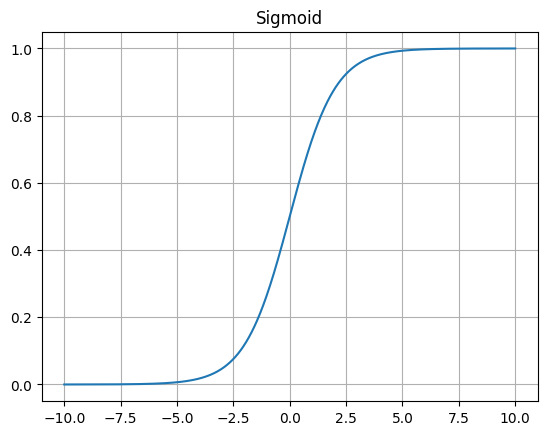
\includegraphics[width=\textwidth]{img/rete/sigmoid.png}
        \caption{Sigmoide}
        \label{fig:sigmoid}
    \end{subfigure}
    \caption{Funzioni di attivazione utilizzate nella fase di grid search}
    \label{fig:}
\end{figure}

Durante il processo di grid search, per ogni modello che è stato addestrato, sono
state raccolte delle informazioni relative all'accuratezza, al tempo di addestramento
richiesto. In aggiunta a queste informazioni, dato che ogni modello è stato
addestrato attraverso una cross validation a 5 fold, sono stati calcolati gli
intervalli di confidenza al $90\%$ per ogni modello addestrato.

Ottenuti i risultati, si è proceduto con l'analisi di questi, in modo tale da
definire la struttura della rete neurale. Per effettuare questa valutazione sono
state utilizzate le misure precedentemente citate.

Il modello selezionato è stato scelto in base al seguente criterio:
\begin{center}
    \textit{Modello = 2 * Accuratezza + 2 * Tempo di addestramento + 1 * Intervalli di confidenza}
\end{center}
Le misure di accuratezza e tempo di addestramento si riferiscono alla media
calcolata attraverso la cross validation.

Nello specifico, sono stati utilizzati i seguenti pesi: 2 per l'accuratezza
media, 2 per il tempo di addestramento medio e 1 per gli intervalli di
confidenza. Questi pesi sono stati scelti in modo tale da dare più importanza
all'accuratezza media e al tempo di addestramento medio, in quanto sono le due
misure che permettono di valutare le prestazioni della rete neurale, mentre gli
intervalli di confidenza sono stati utilizzati per valutare la variabilità delle
prestazioni.

Per verificare la validità del modello scelto si è proceduto con il confronto di
esso con la rete che ha ottenuto la migliore accuratezza e quella che ha ottenuto
il tempo di addestramento minore, ottenendo i risultati riportati in tabella \ref{tab:ris-grid-search}.
\begin{table}[ht]
    \centering
    \begin{tabular}{@{}lcc@{}}
        \toprule
        \rowcolor[HTML]{EFEFEF}
        \multicolumn{1}{c}{\cellcolor[HTML]{EFEFEF}\textbf{Modello}} & \textbf{Accuratezza} & \textbf{Tempo di addestramento} \\ \midrule
        Tempo di addestramento minore                                & 97.9\%               & 1.05s                           \\
        Accuratezza maggiore                                         & 99.0\%               & 14.43s                          \\
        Modello scelto                                               & 98.6\%               & 2.59s                           \\ \bottomrule
    \end{tabular}
    \caption{Risultati ottenuti dalla fase di grid search}
    \label{tab:ris-grid-search}
\end{table}

Dai valori riportati nella tabella \ref{tab:ris-grid-search} si può notare che il
notare che il modello che è stato selezionato fornisce un compromesso tra
accuratezza e tempo di addestramento. Nello specifico, perdendo lo $0.4\%$ di
accuratezza si è ottenuto un tempo di addestramento minore di circa $12$ secondi.
\subsubsection{Definizione della struttura della rete neurale}
Dalla fase di analisi è stato selezionato un sottoinsieme di feature le quali
sono state utilizzate come input della rete neurale. Questo sottoinsieme è
composto da 5 elementi, il che ha permesso di definire la struttura del layer di
input della rete neurale, questo primo strato è composto da 5 neuroni, uno per 
ogni feature selezionata.

I risultati ottenuti dalla fase di grid search hanno permesso di definire la
struttura della rete neurale. In particolare, la rete neurale è composta da 1
layer di input, 2 layer nascosti e 1 layer di output.

I layer nascosti sono composti nel seguente modo:
\begin{itemize}
    \item Il primo layer nascosto è composto da 10 neuroni, in cui la funzione di
          attivazione è la funzione ReLU \ref{fig:relu}.
    \item Il secondo layer nascosto è composto da 5 neuroni, in cui la funzione
          di attivazione è la funzione ReLU \ref{fig:relu}.
\end{itemize}

Per concludere la descrizione della struttura della rete neurale, è necessario
specificare come è composto l'ultimo layer, ovvero quello di output. Vista la
natura del problema di classificazione, il layer di output è composto da un solo
neurone, in cui la funzione di attivazione è la funzione sigmoide \ref{fig:sigmoid}.
\begin{equation}
    \sigma(x) = \frac{1}{1 + e^{-x}}
\end{equation}
Questa scelta è dovuta al fatto che tale funzione restituisce un valore compreso
tra 0 e 1, il che permette di interpretare l'output della rete neurale come la
probabilità che l'input appartenga alla classe positiva.

La struttura della rete neurale è riassunta nella figura \ref{fig:strutturaReteNeurale}.
\begin{figure}[!ht]
    \centering
    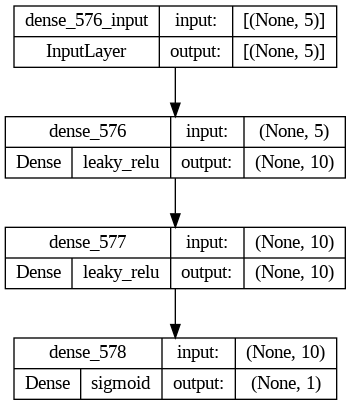
\includegraphics[width=0.3\textwidth]{img/rete/struttura_rete.png}
    \caption{Struttura della rete neurale}
    \label{fig:strutturaReteNeurale}
\end{figure}
\subsubsection{Altri iperparametri} % TODO: titolo migliore
Oltre alla ricerca della struttura della rete neurale, la fase di grid search è
stata utilizzata per valutare l'algoritmo di ottimizzazione, il numero di epoche
e la dimensione del batch.

Per quanto riguarda l'algoritmo di ottimizzazione, il confronto è stato eseguito
tra \textit{Adam} e \textit{SGD}, mentre per il numero di epoche e la dimensione
del batch sono stati valutati i valori 100, 300 per il numero di epoche e 50,
100, 300 per la dimensione del batch.

I risultati ottenuti dalla fase di grid search hanno permesso di definire i valori
degli iperparametri che hanno permesso di ottenere i migliori risultati. In
particolare, l'algoritmo di ottimizzazione scelto è \textit{Adam}, mentre il
numero di epoche e la dimensione del batch sono stati impostati a 100 e 100
rispettivamente.

In questa fase è stato necessario definire la funzione di perdita. Si è scelta
la \textit{binary crossentropy} in quanto adatta a problemi di classificazione
binaria. La scelta di questa loss è dovuta alla natura del problema di
classificazione che si vuole risolvere.
\subsection{Addestramento della rete neurale}
La fase di addestramento della rete neurale è stata effettuata utilizzando il
training set precedentemente definito. L'addestramento della rete neurale è stato
effettuato utilizzando la libreria \textit{Keras} in quanto permette di definire
e addestrare reti neurali in modo intuitivo.
\subsection{Rete neurale su dataset con PCA}
Per verificare se i risultati ottenuti dal modello addestrato sulle feature da
noi selezionate siano effettivamente dovuti alla struttura delle feature e non
a una fortunata selezione, si è deciso di addestrare un modello con le feature
ottenute attraverso la PCA.

Il dataset ottenuto attraverso la PCA, descritto sella sezione \ref{sec:pca}, è
stato diviso in training set e test set in modo tale da mantenere la stessa
percentuale di dati positivi e negativi in entrambi i set. Oltre a questa
operazione, i dati sono stati standardizzati.
Come per il modello addestrato con le feature selezionate manualmente, anche per
questo modello è stata effettuata una fase di grid search per valutare la
combinazione migliore di iperparametri per la rete neurale.

Il processo utilizzato in questa fase è analogo a quello utilizzato per il modello
precedente, sia a livello di iperparametri che di valutazione del modello.

Come fatto in precedenza, il modello selezionato è stato confrontato con il modello
che ha ottenuto la migliore accuratezza e quello che ha ottenuto il tempo di
addestramento minore. I risultati ottenuti sono riportati in tabella \ref{tab:ris-grid-search-pca}.

\begin{table}[ht]
    \centering
    \begin{tabular}{@{}lcc@{}}
        \toprule
        \rowcolor[HTML]{EFEFEF}
        \textbf{Modello}              & \textbf{Accuratezza} & \textbf{Tempo di addestramento} \\ \midrule
        Tempo di addestramento minore & 96.9\%               & 1.06s                           \\
        Accuratezza maggiore          & 98.0\%               & 22.20s                          \\
        Modello scelto                & 97.9\%               & 1.16s                           \\ \bottomrule
    \end{tabular}
    \caption{Risultati ottenuti dalla fase di grid search}
    \label{tab:ris-grid-search-pca}
\end{table}
Anche in questo caso, come per il precedente, il modello che è stato selezionato
rappresenta un compromesso tra accuratezza e tempo di addestramento. In particolare,
perdendo lo $0.1\%$ di accuratezza si è ottenuto un tempo di addestramento minore
di circa $21$ secondi.


I risultati ottenuti dalla fase di grid search hanno permesso di definire la
struttura della rete neurale. In particolare, la rete neurale è composta da 1
layer di input, 1 layer nascosto e 1 layer di output.

Il layer di input è composto da 3 neuroni, uno per ogni componente principale
ottenuta attraverso la PCA. Questo primo strato è stato definito in questo modo
in quanto il dataset ottenuto attraverso la PCA è composto da 3 feature.

Il layer nascosto è composto da 10 neuroni, in cui la funzione di attivazione è
la funzione ReLU \ref{fig:relu}.

Il layer di output è lo stesso utilizzato per il modello addestrato con le feature
selezionate manualmente, ovvero è composto da un solo neurone, in cui la funzione
di attivazione è la funzione sigmoide \ref{fig:sigmoid}.
\begin{figure}[!ht]
    \centering
    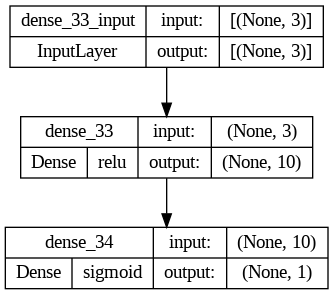
\includegraphics[width=0.3\textwidth]{img/rete/struttura_rete_pca.png}
    \caption{Struttura della rete neurale addestrata con PCA}
    \label{fig:strutturaReteNeuralePCA}
\end{figure}
\chapter{Risultati} \label{chp:risultati}
In questo capitolo verranno presentati i risultati ottenuti dalle due fasi di valutazione
delle diverse versioni dei modelli separati in base ai dataset su cui sono stati 
allenati: \texttt{dataset\_corr} e \texttt{dataset\_pca}. Prima verranno presentati
i risultati ottenuti dalla validazione $80/20$ con gli iperparametri migliori 
ottenuti nel capito precedente

Prima di esporre i risultati ottenuti, è opportuno enunciare la seguente premessa.
Considerando la natura del contesto, mirante alla classificazione di dati medici,
si è convenuto di regolare manualmente il valore della soglia per la predizione
del tumore. Tale decisione è stata presa al fine di minimizzare il numero di
falsi negativi, ossia i casi in cui il modello erroneamente predice l'assenza di
tumore quando invece è presente.

Per effettuare questa operazione, è stato selezionato il valore di soglia pari a
$0.3$, al fine di ridurre il numero di falsi negativi. Questa determinazione è
stata adottata per conferire maggior rilevanza al valore di richiamo, che valuta
l'efficacia del modello nell'individuare i veri positivi.

I classificatori addestrati sono stati valutati mediante l'utilizzo della
porzione di test del dataset. Su questo insieme di dati sono state calcolate le
seguenti metriche di valutazione:

\begin{itemize}
    \item \textbf{Accuracy}: misura la frazione di esempi classificati correttamente.
    \item \textbf{Precision}: misura la frazione di esempi classificati come
          positivi che sono effettivamente positivi.
    \item \textbf{Recall}: misura la frazione di esempi positivi che sono stati
          classificati correttamente.
    \item \textbf{F1-score}: media armonica tra precisione e recall.
\end{itemize}

Oltre a tali metriche, sono state calcolate le matrici di confusione per ciascun
modello e le rispettive curve ROC.

Inoltre, considerando le dimensioni moderate del dataset in esame ($\leq 10000$
esempi), è stato deciso di condurre una valutazione dei modelli utilizzando la
tecnica della $10$-fold stratified cross validation, al fine di ottenere i
valori delle metriche mediante la media dei risultati e i relativi intervalli di
confidenza.

Nelle successive sezioni verranno esposti i risultati ottenuti per ciascun
modello, confrontando i valori delle metriche di valutazione e le curve ROC
generate. I risultati saranno suddivisi in due sezioni, una per il confronto
sul dataset le cui feature sono state selezionate manualmente, una per il
confronto sul dataset le cui feature sono state selezionate con PCA.
\section{Metriche di valutazione \texttt{dataset\_corr}} \label{sec:metriche}
Nella tabella \ref{tab:risultati} sono riportati i valori delle metriche di
valutazione ottenuti per ciascun modello, calcolati sul test set il quale è
composto dal $20\%$ del dataset originale.
\begin{table}[!ht]
    \centering
    \begin{tabular}{@{}cllll@{}}
        \toprule
        \rowcolor[HTML]{EFEFEF}
        \textbf{Modello}                                      & \textbf{Accuratezza}         & \textbf{Precisione}          & \textbf{Richiamo}            & \textbf{F1 score}            \\ \midrule
        \cellcolor[HTML]{EFEFEF}\textbf{SVM}                  & \multicolumn{1}{c}{0 \%}     & \multicolumn{1}{c}{0 \%}     & \multicolumn{1}{c}{0 \%}     & \multicolumn{1}{c}{0 \%}     \\
        \cellcolor[HTML]{EFEFEF}\textbf{Gaussian Naive Bayes} & \multicolumn{1}{c}{95 \%}    & \multicolumn{1}{c}{90 \%}    & \multicolumn{1}{c}{99 \%}    & \multicolumn{1}{c}{94 \%}    \\
        \cellcolor[HTML]{EFEFEF}\textbf{Rete neurale}         & \multicolumn{1}{c}{98.93 \%} & \multicolumn{1}{c}{98.52 \%} & \multicolumn{1}{c}{99.10 \%} & \multicolumn{1}{c}{98.81 \%} \\ \bottomrule
    \end{tabular}
    \caption{Risultati ottenuti dal modello addestrato}
    \label{tab:risultati}
\end{table}

% ! Commento da riguardare e sistemare
I risultati ottenuti rivelano prestazioni superiori per i modelli basati su una
manipolazione geometrica dei dati, come la rete neurale e il Support Vector
Machine (SVM), rispetto al modello fondato su una manipolazione probabilistica,
come il Gaussian Naive Bayes.

Tale fenomeno può essere razionalizzato considerando che le distribuzioni delle
caratteristiche del dataset non rispecchiano una distribuzione gaussiana, come
supposto dal modello Gaussian Naive Bayes. Inoltre, la rete neurale e il SVM
sono modelli intrinsecamente più complessi rispetto al Gaussian Naive Bayes,
consentendo loro di catturare relazioni più intricate tra le caratteristiche e
la variabile target.

In aggiunta, l'ottimo risultato osservato suggerisce una distinta separazione tra le
due classi del dataset, suggerendo che i modelli sono capaci di generalizzare
efficacemente.

Il comportamento osservato dalle metriche può essere visualizzato mediante le
matrici di confusione, sulle quali le metriche presentate vengono calcolate, le
quali sono riportate in figura \ref{fig:matrice_di_confusione_per_SVM_corr},
\ref{fig:matrice_di_confusione_per_GNB_corr} e \ref{fig:matrice_di_confusione_per_NN_corr}.
\begin{figure}[!ht]
    \centering
    \begin{subfigure}{0.45\textwidth}
        \centering
        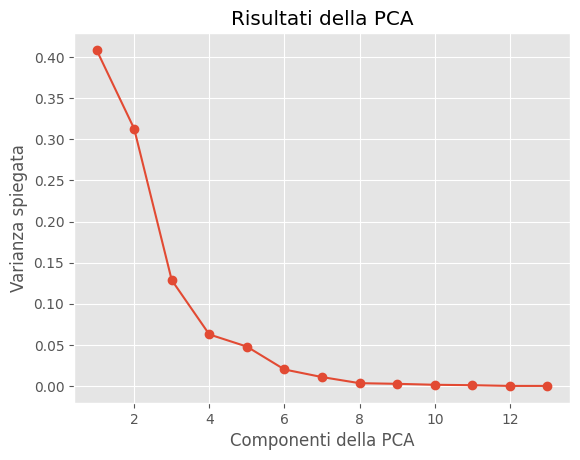
\includegraphics[width=\textwidth]{img/analisi/pcaVarianza.png}
        \caption{Support Vector Machine}
        \label{fig:matrice_di_confusione_per_SVM_corr}
    \end{subfigure}
    \hfill
    \begin{subfigure}{.45\textwidth}
        \centering
        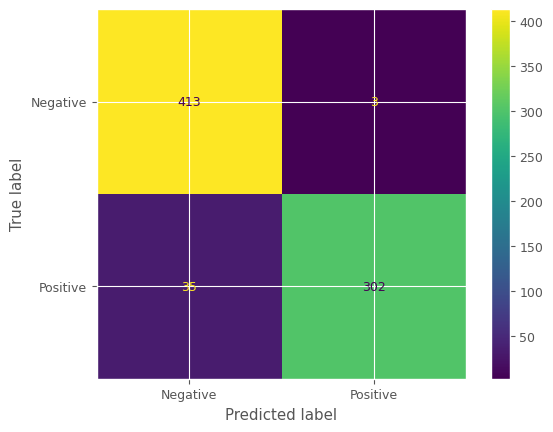
\includegraphics[width=\textwidth]{img/gnb/confusion_matrix_corr.png}
        \caption{Gaussian Naive Bayes}
        \label{fig:matrice_di_confusione_per_GNB_corr}
    \end{subfigure}
    \hfill
    \begin{subfigure}{.45\textwidth}
        \centering
        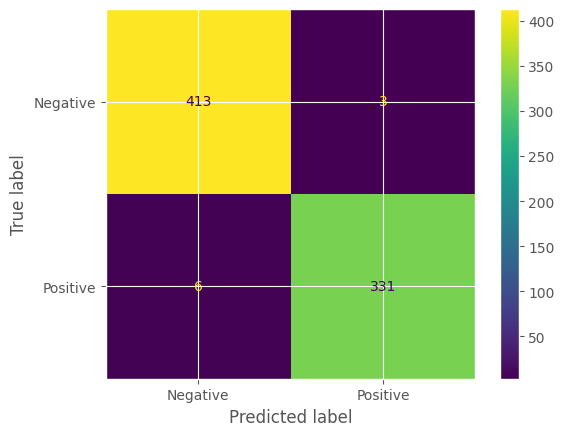
\includegraphics[width=\textwidth]{img/rete/matrice_confusione.png}
        \caption{Rete neurale}
        \label{fig:matrice_di_confusione_per_NN_corr}
    \end{subfigure}
    \caption{Matrici di confusione per i modelli addestrati su \texttt{dataset\_corr} e \texttt{dataset\_corr\_std}}
    \label{fig:matrice_di_confusione_per_corr}
\end{figure}
% TODO: Creare le immagini nuove per le matrici di confusione senza griglia

\subsection{Curve ROC} \label{subsec:roc}
In aggiunta alla valutazione delle performance tramite le metriche, si è deciso
di confrontare i modelli attraverso le curve ROC, le quali permettono di
confrontare i modelli in termini di trade-off tra tasso di veri positivi e tasso
di falsi positivi.

Le curve ROC per i modelli addestrati sul dataset le cui feature sono state
selezionate manualmente sono riportate in figura \ref{fig:roc_curve_corr}.

\begin{figure}[!ht]
    \centering
    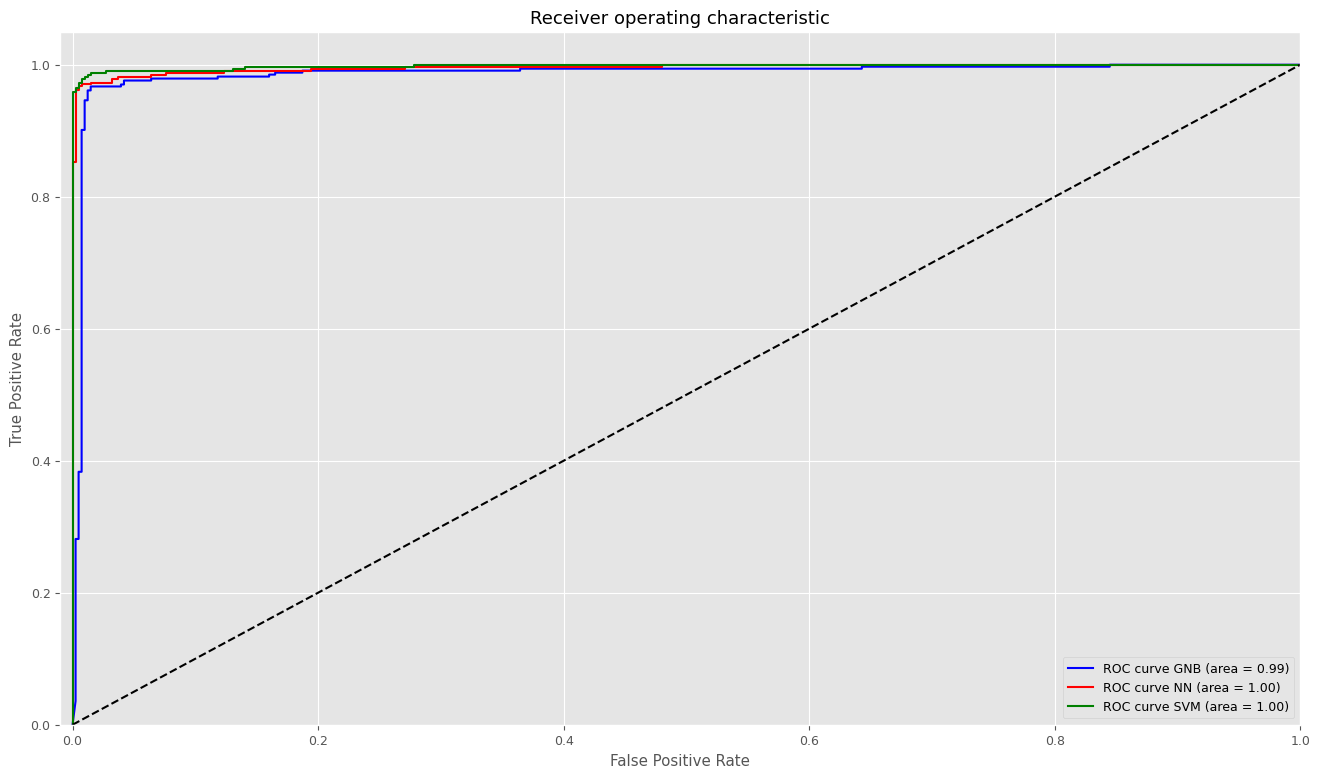
\includegraphics[width=\textwidth]{img/ris/roc_curve_corr.png}
    \caption{Curve ROC per i modelli addestrati su \texttt{dataset\_corr} e \texttt{dataset\_corr\_std}}
    \label{fig:roc_curve_corr}
\end{figure}

Le curve ROC permettono di confrontare i modelli addestrati anche con il classificatore
casuale, il quale corrisponde alla retta $y = x$. Il grafico riportato in figura
\ref{fig:roc_curve_corr} mostra che la rete neurale e il Gaussian Naive Bayes
hanno delle prestazioni molto simili tra loro, è quindi utile confrontare i due
due tramite l'area sotto la curva ROC (AUC). L'area sotto la curva ROC
per la rete neurale è pari a $1.00$, mentre per il Gaussian Naive Bayes è pari a
$0.99$. Questi valori suggeriscono che la rete neurale è leggermente superiore
al Gaussian Naive Bayes in termini di capacità di discriminazione tra le due
classi.

\subsection{10 fold stratified cross validation} \label{subsec:cross_val}
Per valutare la stabilità dei modelli addestrati e date le dimensioni moderate del
dataset, si è deciso di condurre una valutazione tramite la tecnica della
$10$-fold stratified cross validation. Tale tecnica permette di ottenere una
stima più accurata delle performance del modello, riducendo l'effetto della
variabilità dei dati.

In questo processo ogni modello che è stato addestrato è stato valutato attraverso
le metriche di accuratezza, precisione, richiamo e F1 score. I risultati ottenuti
dall'esecuzione della cross validation sono stati utilizzati per calcolare gli
intervalli di confidenza al $90\%$ delle metriche.

Per svolgere questa operazione è stato utilizzato il dataset completo, ovvero
senza alcuna suddivisione in training set e test set.

I risultati ottenuti sono stati riportati sia in forma numerica che grafica
per facilitare la comprensione. In particolare, i valori delle metriche ottenuti
sono stati riportati in figura \ref{fig:intervalli_confidenza_corr} e
nella tabella \ref{tab:intervalli_confidenza_corr}.

\begin{table}[!ht]
    \begin{subtable}[h]{1\textwidth}
        \centering
        \begin{tabular}{@{}cllll@{}}
            \toprule
            \rowcolor[HTML]{EFEFEF}
            \textbf{Modello}                                      & \textbf{Accuratezza}         & \textbf{Precisione}          & \textbf{Richiamo}            & \textbf{F1 score}            \\ \midrule
            \cellcolor[HTML]{EFEFEF}\textbf{SVM}                  & \multicolumn{1}{c}{0 \%}     & \multicolumn{1}{c}{0 \%}     & \multicolumn{1}{c}{0 \%}     & \multicolumn{1}{c}{0 \%}     \\
            \cellcolor[HTML]{EFEFEF}\textbf{Gaussian Naive Bayes} & \multicolumn{1}{c}{95 \%}    & \multicolumn{1}{c}{90 \%}    & \multicolumn{1}{c}{99 \%}    & \multicolumn{1}{c}{94 \%}    \\
            \cellcolor[HTML]{EFEFEF}\textbf{Rete neurale}         & \multicolumn{1}{c}{98.27 \%} & \multicolumn{1}{c}{97.99 \%} & \multicolumn{1}{c}{98.15 \%} & \multicolumn{1}{c}{98.06 \%} \\ \bottomrule
        \end{tabular}
        \caption{Valore medio delle metriche ottenute dalla cross validation}
        \label{tab:risultati_cross_val_corr}
    \end{subtable}
    \hfill
    \begin{subtable}[h]{1\textwidth}
        \centering
        \begin{tabular}{@{}cllll@{}}
            \toprule
            \rowcolor[HTML]{EFEFEF}
            \textbf{Modello}                                      & \textbf{Accuratezza} & \textbf{Precisione} & \textbf{Richiamo}  & \textbf{F1 score}  \\ \midrule
            \cellcolor[HTML]{EFEFEF}\textbf{SVM}                  & []                   & []                  & []                 & []                 \\
            \cellcolor[HTML]{EFEFEF}\textbf{Gaussian Naive Bayes} & []                   & []                  & []                 & []                 \\
            \cellcolor[HTML]{EFEFEF}\textbf{Rete neurale}         & [97.98\%, 98.55\%]   & [97.47\%, 98.52\%]  & [97.49\%, 98.81\%] & [97.75\%, 98.38\%] \\ \bottomrule
        \end{tabular}
        \caption{Intervalli di confidenza delle metriche ottenute dalla cross validation}
        \label{tab:intervalli_confidenza_corr}
    \end{subtable}
    \caption{Risultati ottenuti dalla cross validation}
    \label{tab:intervalli_confidenza_corr}
\end{table}
% TODO: cambiare le immagini con quelle nuove
\begin{figure}[!ht]
    \centering
    \begin{subfigure}[b]{0.4\textwidth}
        \centering
        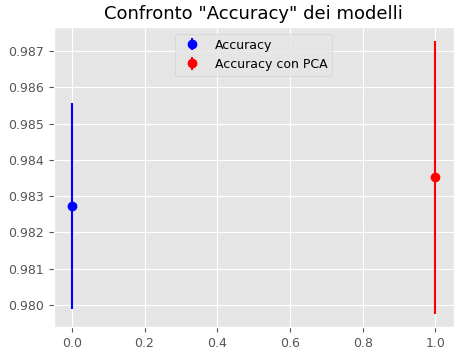
\includegraphics[width=\textwidth]{img/rete/intervalliAcc.png}
        \caption{Accuracy}
        \label{fig:acc}
    \end{subfigure}
    \hfill
    \begin{subfigure}[b]{0.4\textwidth}
        \centering
        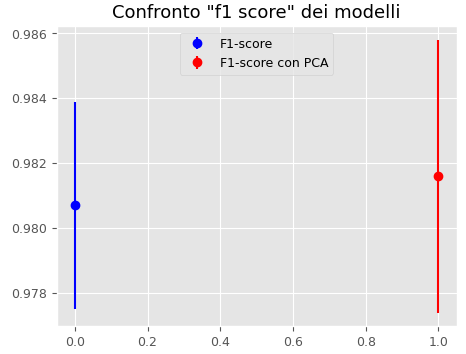
\includegraphics[width=\textwidth]{img/rete/intervalliF1.png}
        \caption{F1 score}
        \label{fig:f1}
    \end{subfigure}
    \hfill
    \begin{subfigure}[b]{0.4\textwidth}
        \centering
        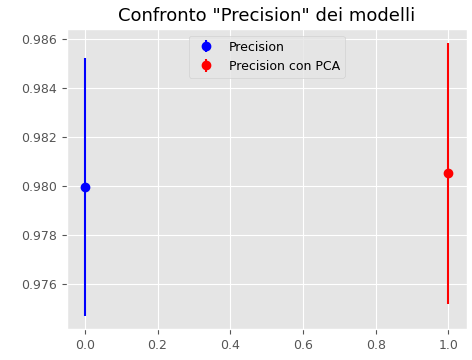
\includegraphics[width=\textwidth]{img/rete/intervalliPrecision.png}
        \caption{Precision}
        \label{fig:precision}
    \end{subfigure}
    \hfill
    \begin{subfigure}[b]{0.4\textwidth}
        \centering
        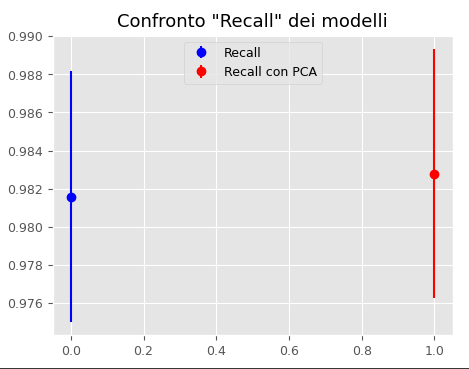
\includegraphics[width=\textwidth]{img/rete/intervalliRecall.png}
        \caption{Recall}
        \label{fig:recall}
    \end{subfigure}
    \caption{Intervalli di confidenza ottenuti dai modelli addestrati con e senza PCA}
    \label{fig:intervalli_confidenza_corr}
\end{figure}

% ! Commento sugli intervalli di confidenza e confronto con i valori ottenuti

\section{Metriche di valutazione \texttt{dataset\_pca}} \label{sec:metriche_pca}
Un ragionamento analogo a quello svolto nella sezione \ref{sec:metriche} può essere
applicato ai modelli addestrati sul dataset le cui feature sono state selezionate
attraverso Principal Component Analysis (PCA). I risultati ottenuti sono riportati
nella tabella \ref{tab:risultati_pca}.

\begin{table}[!ht]
    \centering
    \begin{tabular}{@{}cllll@{}}
        \toprule
        \rowcolor[HTML]{EFEFEF}
        \textbf{Modello}                                      & \textbf{Accuratezza}         & \textbf{Precisione}          & \textbf{Richiamo}            & \textbf{F1 score}            \\ \midrule
        \cellcolor[HTML]{EFEFEF}\textbf{SVM}                  & \multicolumn{1}{c}{0 \%}     & \multicolumn{1}{c}{0 \%}     & \multicolumn{1}{c}{0 \%}     & \multicolumn{1}{c}{0 \%}     \\
        \cellcolor[HTML]{EFEFEF}\textbf{Gaussian Naive Bayes} & \multicolumn{1}{c}{96 \%}    & \multicolumn{1}{c}{96 \%}    & \multicolumn{1}{c}{96 \%}    & \multicolumn{1}{c}{96 \%}    \\
        \cellcolor[HTML]{EFEFEF}\textbf{Rete neurale}         & \multicolumn{1}{c}{98.27 \%} & \multicolumn{1}{c}{97.92 \%} & \multicolumn{1}{c}{98.21 \%} & \multicolumn{1}{c}{98.07 \%} \\ \bottomrule
    \end{tabular}
    \caption{Risultati ottenuti dal modello addestrato}
    \label{tab:risultati_pca}
\end{table}

I risultati ottenuti rivelano prestazioni molto simili con quelle ottenute per il
dataset le cui feature sono state selezionate manualmente.

Come fatto in precedenza, è possibile visualizzare il comportamento dei modelli
mediante le matrici di confusione, le quali sono riportate in figura \ref{fig:matrice_di_confusione_per_SVM_pca},
\ref{fig:matrice_di_confusione_per_GNB_pca} e \ref{fig:matrice_di_confusione_per_NN_pca}.

\begin{figure}[!ht]
    \centering
    \begin{subfigure}{0.45\textwidth}
        \centering
        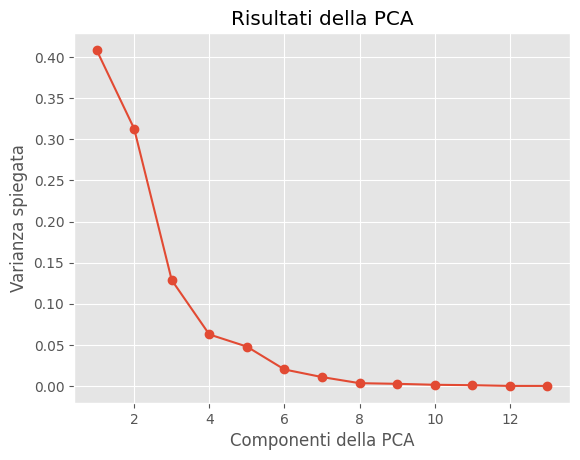
\includegraphics[width=\textwidth]{img/analisi/pcaVarianza.png}
        \caption{Support Vector Machine}
        \label{fig:matrice_di_confusione_per_SVM_pca}
    \end{subfigure}
    \hfill
    \begin{subfigure}{.45\textwidth}
        \centering
        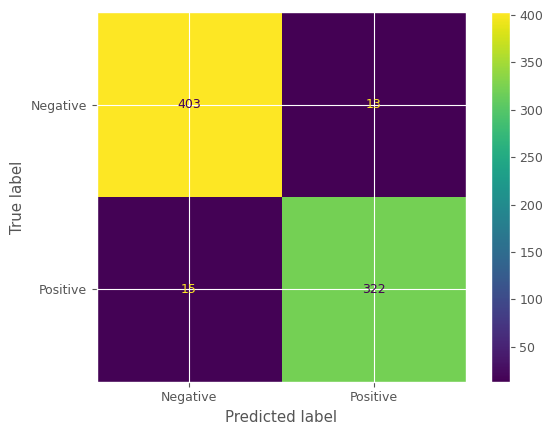
\includegraphics[width=\textwidth]{img/gnb/confusion_matrix_pca.png}
        \caption{Gaussian Naive Bayes}
        \label{fig:matrice_di_confusione_per_GNB_pca}
    \end{subfigure}
    \hfill
    \begin{subfigure}{.45\textwidth}
        \centering
        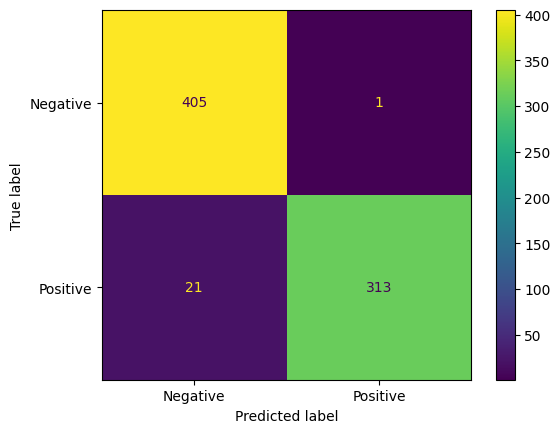
\includegraphics[width=\textwidth]{img/rete/matrice_confusione_PCA.png}
        \caption{Rete neurale}
        \label{fig:matrice_di_confusione_per_NN_pca}
    \end{subfigure}
    \caption{Matrici di confusione per i modelli addestrati su \texttt{dataset\_pca} e \texttt{dataset\_pca\_std}}
    \label{fig:matrice_di_confusione_per_pca}
\end{figure}

Inoltre, anche in questo caso, è possibile confrontare i modelli attraverso le curve
ROC, le quali sono riportate in figura \ref{fig:roc_curve_pca}.
\begin{figure}[!ht]
    \centering
    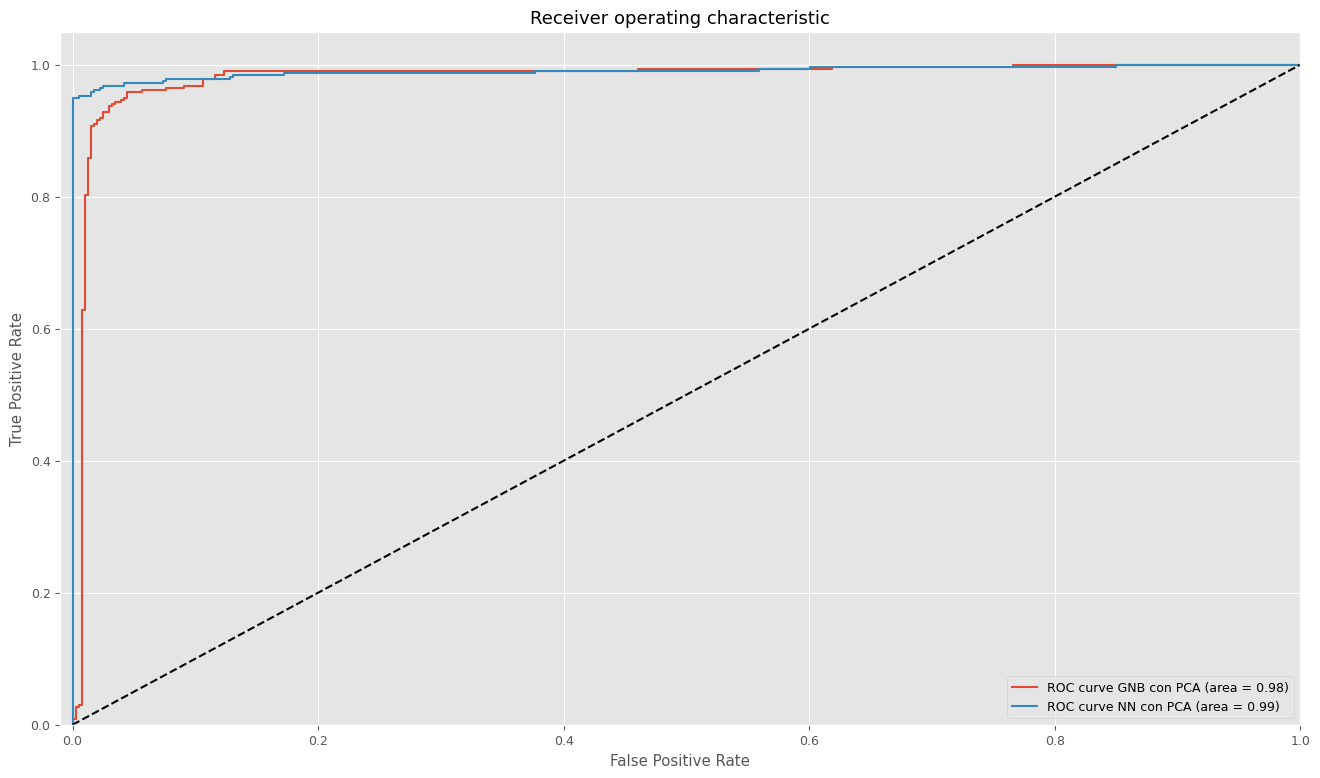
\includegraphics[width=\textwidth]{img/ris/roc_curve_pca.png}
    \caption{Curve ROC per i modelli addestrati su \texttt{dataset\_pca} e \texttt{dataset\_pca\_std}}
    \label{fig:roc_curve_pca}
\end{figure}

Utilizzando la PCA per la creazione del dataset nelle curve ROC si può notare
una maggiore distanza tra la curva ROC della rete neurale e quella del Gaussian
Naive Bayes. Inoltre, calcolando l'area sotto la curva ROC (AUC) si può notare
come la rete neurale sia leggermente superiore al Gaussian Naive Bayes, con un
valore di $0.99$ per la rete neurale e di $0.98$ per il Gaussian Naive Bayes. Il
che suggerisce che questi classificatori sono leggermente peggiori rispetto a
quelli addestrati sul dataset le cui feature sono state selezionate manualmente.

Infine, per restare coerenti con quanto fatto in precedenza, è possibile valutare
la stabilità dei modelli addestrati tramite la tecnica della $10$-fold stratified
cross validation. I risultati ottenuti sono riportati in figura \ref{fig:intervalli_confidenza_pca}
e nella tabella \ref{tab:intervalli_confidenza_pca}.

\begin{table}[!ht]
    \begin{subtable}[h]{1\textwidth}
        \centering
        \begin{tabular}{@{}cllll@{}}
            \toprule
            \rowcolor[HTML]{EFEFEF}
            \textbf{Modello}                                      & \textbf{Accuratezza}         & \textbf{Precisione}          & \textbf{Richiamo}            & \textbf{F1 score}            \\ \midrule
            \cellcolor[HTML]{EFEFEF}\textbf{SVM}                  & \multicolumn{1}{c}{0 \%}     & \multicolumn{1}{c}{0 \%}     & \multicolumn{1}{c}{0 \%}     & \multicolumn{1}{c}{0 \%}     \\
            \cellcolor[HTML]{EFEFEF}\textbf{Gaussian Naive Bayes} & \multicolumn{1}{c}{96 \%}    & \multicolumn{1}{c}{96 \%}    & \multicolumn{1}{c}{96 \%}    & \multicolumn{1}{c}{96 \%}    \\
            \cellcolor[HTML]{EFEFEF}\textbf{Rete neurale}         & \multicolumn{1}{c}{98.35 \%} & \multicolumn{1}{c}{98.05 \%} & \multicolumn{1}{c}{98.27 \%} & \multicolumn{1}{c}{98.15 \%} \\ \bottomrule
        \end{tabular}
        \caption{Valore medio delle metriche ottenute dalla cross validation}
        \label{tab:risultati_cross_val_pca}
    \end{subtable}
    \hfill
    \begin{subtable}[h]{1\textwidth}
        \centering
        \begin{tabular}{@{}cllll@{}}
            \toprule
            \rowcolor[HTML]{EFEFEF}
            \textbf{Modello}                                      & \textbf{Accuratezza} & \textbf{Precisione} & \textbf{Richiamo}  & \textbf{F1 score}  \\ \midrule
            \cellcolor[HTML]{EFEFEF}\textbf{SVM}                  & []                   & []                  & []                 & []                 \\
            \cellcolor[HTML]{EFEFEF}\textbf{Gaussian Naive Bayes} & []                   & []                  & []                 & []                 \\
            \cellcolor[HTML]{EFEFEF}\textbf{Rete neurale}         & [97.97\%, 98.72\%]   & [97.51\%, 98.58\%]  & [97.62\%, 98.93\%] & [97.73\%, 98.58\%] \\ \bottomrule
        \end{tabular}
        \caption{Intervalli di confidenza delle metriche ottenute dalla cross validation}
        \label{tab:intervalli_confidenza_pca}
    \end{subtable}
    \caption{Risultati ottenuti dalla cross validation}
    \label{tab:intervalli_confidenza_pca}
\end{table}

% TODO: Sono da calcolare e inserire
\begin{figure}[!ht]
    \centering
    \begin{subfigure}[b]{0.4\textwidth}
        \centering
        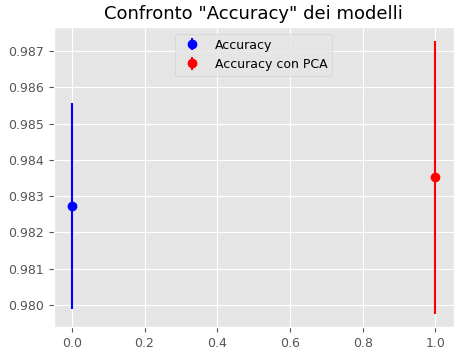
\includegraphics[width=\textwidth]{img/rete/intervalliAcc.png}
        \caption{Accuracy}
        \label{fig:acc_pca}
    \end{subfigure}
    \hfill
    \begin{subfigure}[b]{0.4\textwidth}
        \centering
        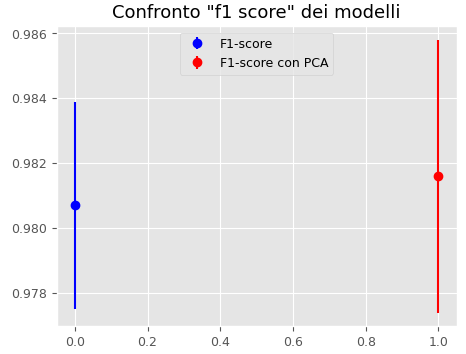
\includegraphics[width=\textwidth]{img/rete/intervalliF1.png}
        \caption{F1 score}
        \label{fig:f1_pca}
    \end{subfigure}
    \hfill
    \begin{subfigure}[b]{0.4\textwidth}
        \centering
        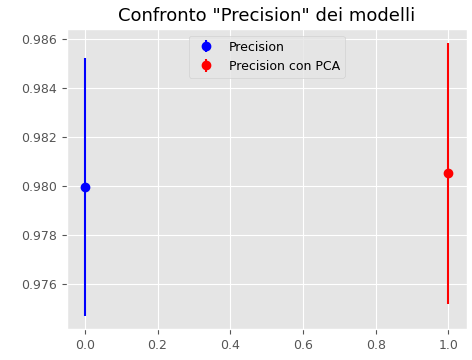
\includegraphics[width=\textwidth]{img/rete/intervalliPrecision.png}
        \caption{Precision}
        \label{fig:precision_pca}
    \end{subfigure}
    \hfill
    \begin{subfigure}[b]{0.4\textwidth}
        \centering
        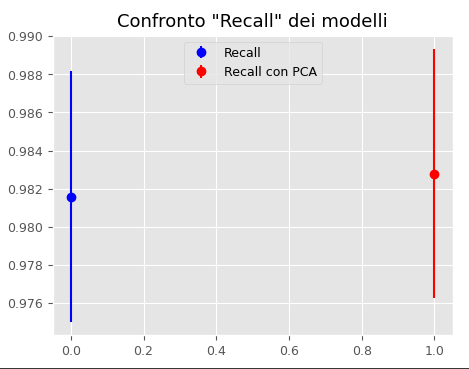
\includegraphics[width=\textwidth]{img/rete/intervalliRecall.png}
        \caption{Recall}
        \label{fig:recall_pca}
    \end{subfigure}
    \caption{Intervalli di confidenza ottenuti dai modelli addestrati con e senza PCA}
    \label{fig:intervalli_confidenza_pca}
\end{figure}

% ! Commento dei risultati da fare
\chapter{Conclusioni}
L'intero progetto si è basato sul riconoscimento della presenza del tumore del
cervello a partire da immagini in bianco e nero prodotte dalla risonanza
magnetica dei pazienti.

Prima di tutto, è stato chiarito il processo di estrazione delle caratteristiche
dalle immagini della risonanza magnetica. Ciò ha consentito di comprendere il
significato delle caratteristiche calcolate, un passaggio fondamentale per
analizzare in dettaglio tutte le analisi esplorative condotte sul dataset.

Esaminata la composizione del dataset, è stata condotta un'analisi esplorativa
durante la quale sono state applicate varie trasformazioni per eliminare
eventuali valori nulli o costanti. Successivamente, si è proseguito valutando
l'equilibrio delle classi nel dataset e analizzando le distribuzioni delle
feature attraverso una rappresentazione grafica. Da queste indagini è emerso che
le classi presenti nel dataset sono bilanciate e che alcuni attributi non presentano
una distribuzione normale.

In seguito all'analisi delle distribuzioni, sono stati generati box plot per
ciascuna caratteristica, distinguendo tra le due classi del dataset. Questo
approccio ha consentito di identificare eventuali attributi costanti e
caratteristiche altamente discriminanti.

Durante l'analisi esplorativa, sono stati condotti studi sulle correlazioni tra
le caratteristiche al fine di identificare possibili relazioni tra gli attributi.
Da questa fase è emerso che diverse correlazioni sono presenti tra le
caratteristiche che misurano la distribuzione dei livelli di grigio e quelle
legate alla valutazione del contrasto e dell'omogeneità delle texture.

Successivamente, al termine dell'analisi esplorativa, è stata necessaria una
riduzione della dimensionalità prima di fornire i dati agli algoritmi di machine
learning. Notando le correlazioni tra gli attributi, si è deciso di non limitarsi
alla sola riduzione dimensionale con l'analisi delle componenti principali (PCA),
ma di considerare anche la rimozione delle correlazioni. Di conseguenza, sono
stati creati due dataset distinti: \texttt{dataset\_corr} e \texttt{dataset\_pca},
al fine di confrontare non solo i modelli, ma anche i due metodi di riduzione
dimensionale.

Dopo la creazione dei due dataset ridotti, sono stati valutati i modelli
selezionati su entrambi. La valutazione è stata suddivisa in due fasi:
\begin{itemize}
    \item La prima consisteva nella divisione di ciascun dataset in train e test
          per l'allenamento e la valutazione dei modelli.
    \item La seconda fase ha coinvolto una cross-validation per calcolare gli
          intervalli di confidenza delle metriche.
\end{itemize}
Per i modelli che richiedevano l'ottimizzazione degli iperparametri, questa è
stata eseguita tramite cross-validation sul train set della prima valutazione,
utilizzando gli stessi iperparametri per la seconda valutazione.

In merito ai risultati ottenuti dalla valutazione dei modelli, emerge che tutti
e tre i modelli sono efficaci classificatori per il problema, con valori
superiori al $90\%$ per ogni metrica di valutazione. Un'analisi più approfondita
mostra che la metodologia di riduzione della dimensionalità ha un impatto
limitato sui risultati, con metriche e intervalli molto simili sia nella prima
che nella seconda valutazione. Si osserva però un miglioramento dal punto di
vista computazionale, con tempi di addestramento inferiori per i modelli addestrati.

Tra i modelli, la rete neurale e il SVM si distinguono per le loro prestazioni
superiori, mentre per quanto riguarda Gaussian Naive Bayes non si riescono a
raggiunge gli stessi risultati, specialmente per la Recall, la quale è la metrica
più importante nel contesto del problema di classificazione dei tumori. Questo
perché è preferibile avere un falso positivo piuttosto che un falso negativo,
in quanto un falso negativo potrebbe portare a non diagnosticare la presenza di
un tumore.

In conclusione, tutti e tre i modelli si sono dimostrati validi per la
classificazione dei tumori. Tuttavia, i risultati indicano che il modello SVM
eccelle in termini di precisione e efficienza temporale rispetto alla rete
neurale, considerando anche i tempi di addestramento e di ottimizzazione degli
iperparametri, che si sono rivelati inferiori per SVM.
\chapter*{Appendice}
\begin{figure}[!ht]
    \centering
    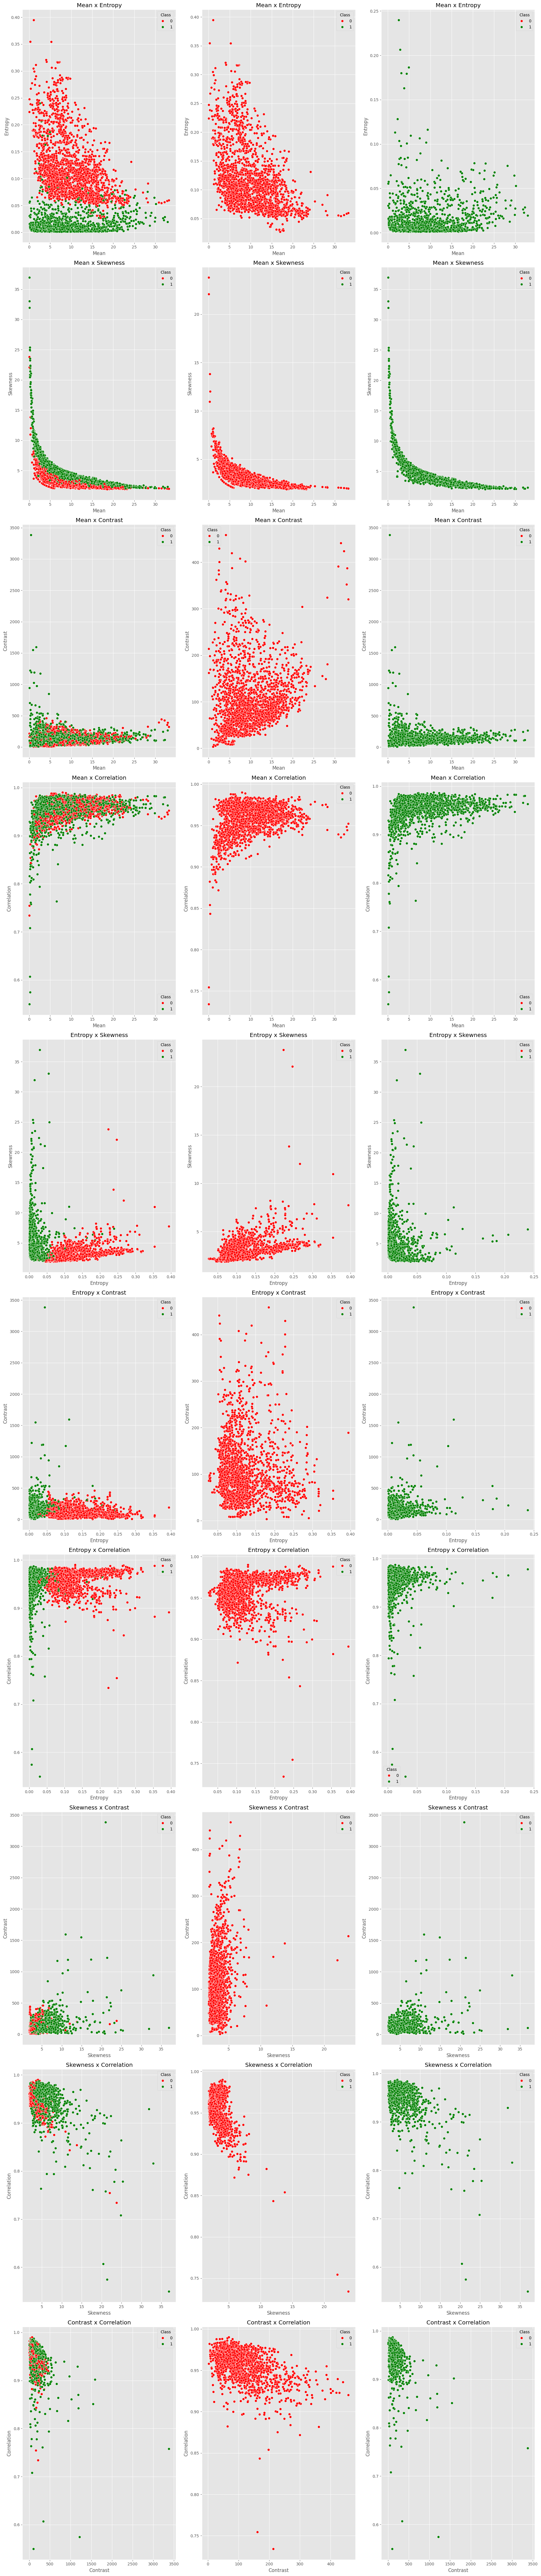
\includegraphics[height=0.95\textheight]{img/analisi/scatterplot.png}
    \caption{Scatterplot di tutte le combinazioni di features}
    \label{fig:scatterplot_features}
\end{figure}

\bibliographystyle{unsrt}
\bibliography{bibliography}

\end{document}